\subsection{Pantalla: Consultar Estudios.}

\subsubsection{Objetivo}
	El mapa de navegación se muestra en la Figura~\ref{fig:mapaNavegacionCU1}

 %  \begin{figure}[hbpt!]
% 		\centering
% 			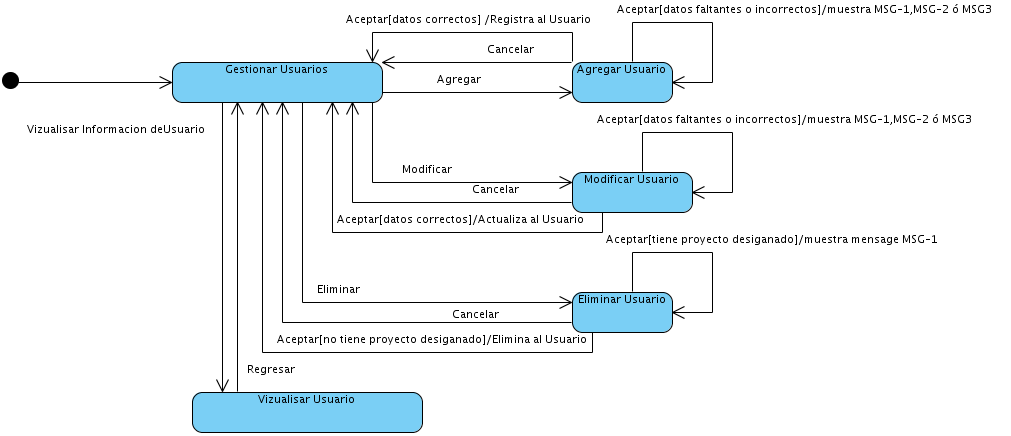
\includegraphics[width=0.8\textwidth]{images/CU1/NavegacionUsuarios.png}
% 		\caption{Mapa de navegacion para el CUE2 Consultar Estudios.}%
%		\label{fig:mapaNavegacionCU1}
% 	\end{figure}

\subsubsection{Objetivo}
Mostrar el menú para consultar un estudio ya sea por Eje Temático o por Tema Transeversal.
Figura~\ref{IUGestUsuarios}

\IUfig[0.6]{CUE2/ConsultarEstudios.png}{IUConsultarEstudios}{Pantalla: Consultar Estudios.}
\subsubsection{Salidas}
Se muestra la lista de los Estudios registrados, ordenados por nombre.
\subsubsection{Controles}
\begin{itemize}
 \item \IUbutton{Flecha derecha} Muestra los siguientes n estudios.
 \item \IUbutton{Flecha izquierda} Muestra los n estudios anteriores.
\end{itemize}

\subsubsection{Comandos}
\begin{itemize}
 \item \IUbutton{Consultar por Eje Temático} Permite consultar un estudio por Eje Temático, Muestra la pantalla \IUref{IUConsultarPorEje}{Consultar por Eje Temático}.
 \item \IUbutton{Consultar por Tema Transversal} Permite consultar un estudio por Tema Transversal, Muestra la pantalla.\IUref{IUConsultarPorTema}{Consultar por Tema Transversal}.

\end{itemize}


